\chapter{数据分析}

\def\la{\langle}
\def\ra{\rangle}
\cite{Abbott2020} (翻译见 \texttt{others/data\_{}analysis/}). \cite{Maggiore2014}, \cite{Jaranowski2012,Jaranowski2009}, \cite{Finn1992}, \cite{Thrane2019}.

\section{主要步骤}

\begin{figure}[htbp]
    \centering
    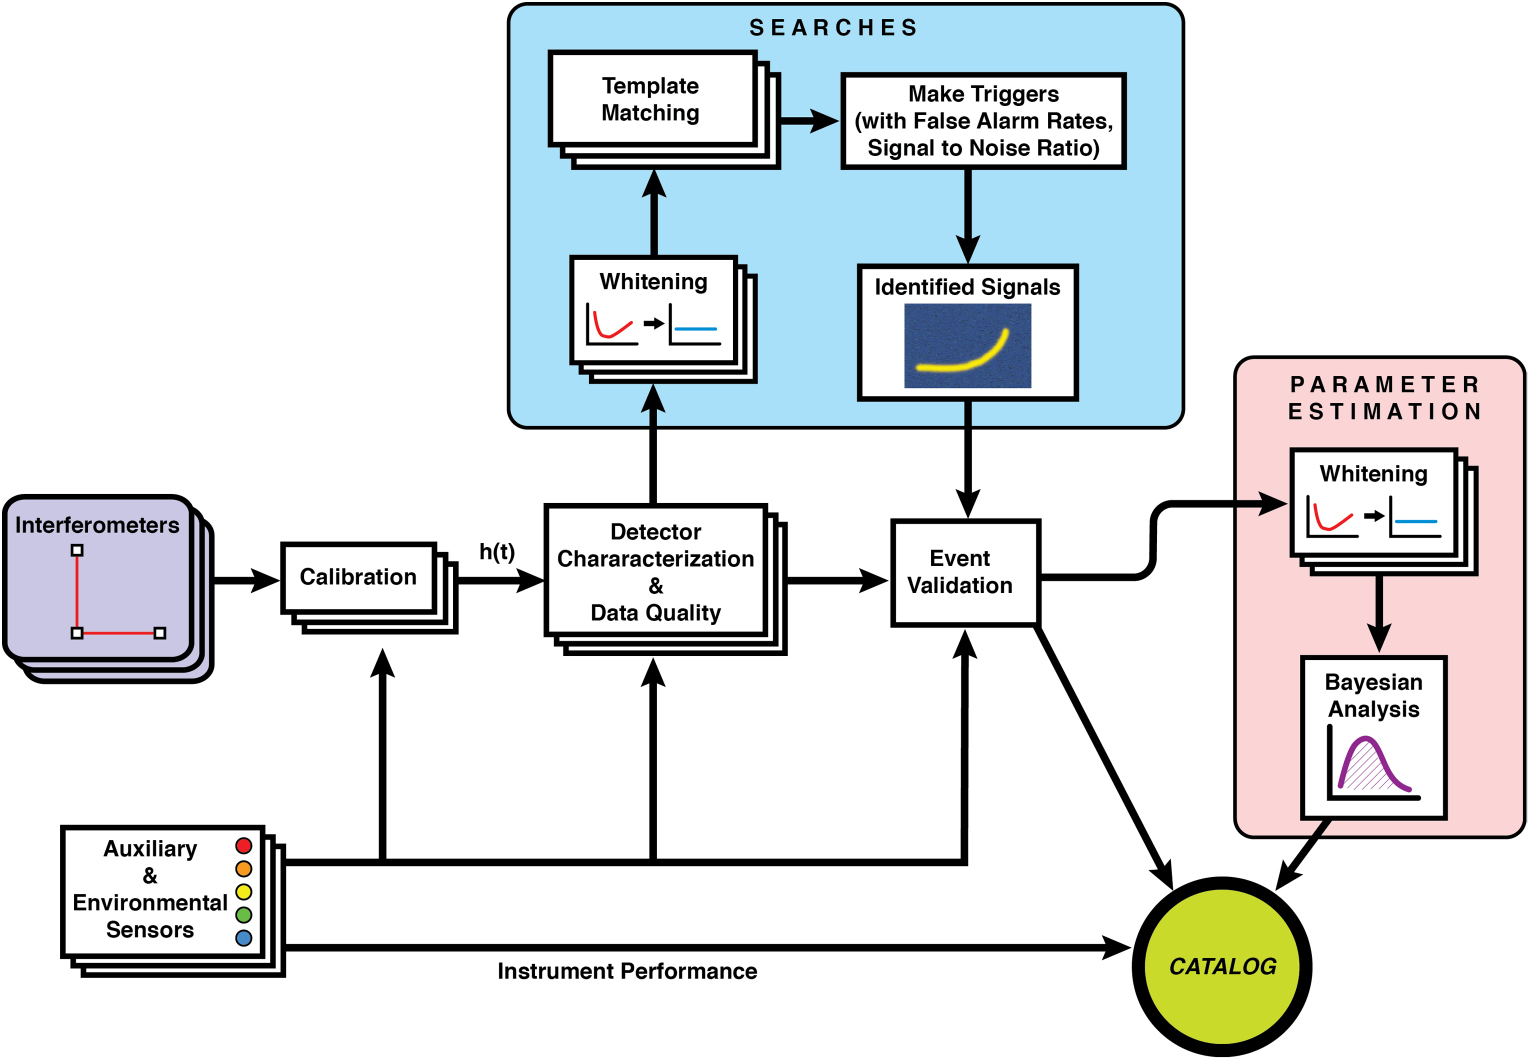
\includegraphics[width=\textwidth]{image/data_processing_main_steps.jpg}
    \caption{
        一个简化的示意图, 总结 LIGO-Virgo 数据处理的主要步骤, 从数据输出到瞬态事件表中报告的结果. 
    }
\end{figure}

\section{定义}

简单认为
\begin{equation}
    S_t=h(t)+N_t
\end{equation}
详细讨论见 \cite{Maggiore2014}.

内积
\begin{equation}
    \la p\mid q \ra:=4\text{Re}\int_0^\infty\frac{\tilde{p}^*(f)\tilde{q}(f)}{S_{N}(f)}\,\d f.
\end{equation}

\section{PSD}

\begin{equation}
    R(\tau):=\text{E}(N_tN_{t+\tau}),
\end{equation}
\begin{equation}
    \frac{1}{2}S_{N}(f):=S_{N}^\t{双边}(f):=\tilde{R}(f):=\int R(\tau)e^{i2\pi f\tau}\,\d\tau.
\end{equation}

若 $\tilde{N}_f$ 存在, 则
\begin{equation}
    \text{E}(N_f^*N_{f'})=\delta(f-f')S_{N}^\t{双边}(f).
\end{equation}

\section{Matched filtering}

\begin{equation}
    \mathcal{S}(K):=\int S_tK(t)\,\d t
\end{equation}
\begin{equation}
    \mathcal{N}(K):=\int N_tK(t)\,\d t
\end{equation}
\begin{align}
    \frac{\mathrm{S}}{\mathrm{N}}(K)&:=\frac{\text{E}(\mathcal{S})}{\sqrt{\text{D}(\mathcal{N})}}\\
    &=\frac{\text{E}(\int S_tK(t)\,\d t)}{\sqrt{\text{D}(\int N_tK(t)\,\d t)}}\\
    &=\frac{\int h(t)K(t)\,\d t}{\sqrt{\int \text{E}(N_{t_1}N_{t_2})K(t_1)K(t_2)\,\d t_1\d t_2}}\\
    &=\frac{\int h(t)K(t)\,\d t}{\sqrt{\int R(t_2-t_1)K(t_1)K(t_2)\,\d t_1\d t_2}}\\
    &=\frac{\int \ti{h}(f)\ti{K}^*(f)\,\d f}{\sqrt{\int\frac{1}{2}S_{N}(f)\ti{K}(f)\ti{K}^*(f)\,\d f}}\\
    &=\frac{\la \frac{1}{2}S_{N}\ti{K}\mid h \ra}{\la \frac{1}{2}S_{N}\ti{K}\mid \frac{1}{2}S_{N}\ti{K} \ra^{1/2}}
\end{align}
\begin{equation}
    \max{[\frac{\mathrm{S}}{\mathrm{N}}(K)]}=\la h\mid h \ra^{1/2}
\end{equation}

\section{Event validation}

\begin{equation}
    \rho:=\frac{\mathcal{S}}{\mathrm{N}}(K)
\end{equation}
When $h=0$,
\begin{equation}
    \rho=\frac{\mathcal{N}}{\mathrm{N}}(K)
\end{equation}
Since $N_t$ is Gaussian, $\mathcal{N}(K)=\int N_tK(t)\,\d t$ is Gaussian,
\begin{equation}
    p(\rho|0)=\frac{1}{\sqrt{2\pi}}e^{-\rho^2/2}\,\d\rho,
\end{equation}
\begin{equation}
    p_{\t{FA}}=2\erfc{\rho_\t{t}/\sqrt{2}}.
\end{equation}
\begin{theorem}
    事件 $A_1,\dots,A_n$, $\eta$ 是 $A_1,\dots,A_n$中事件的发生数, 则$\text{E}(\eta)=\sum_{i=1}^nP(A_i)$.
\end{theorem}
\begin{proof}
    $\eta=\sum_{i=1}^n\t{I}_{A_i}$, $\t{E}(\eta)=\int\eta\,\d P=\sum_{i=1}^n\int\t{I}_{A_i}\,\d P=\sum_{i=1}^nP(A_i)$.
\end{proof}

\section{Parameter estimation}

\begin{equation}
    p(\mu\mid d)\propto p(\mu)\exp\left[-\frac{1}{2}\sum_{m,n}C_{mn}^{-1}(d_m-h_m)(d_n-h_n)\right],
\end{equation}
\begin{equation}
    p(\mu\mid d)\propto p(\mu)\exp\left[-\frac{1}{2}\la d-h\mid d-h \ra\right].
\end{equation}

\section{Sensitivity}

Fisher information matrix
\begin{equation}
    \Gamma_{mn}:=\text{E}(\p_m \ln p\,\p_n \ln p),
\end{equation}
$p=p(s|\vec{\theta})=\Lambda(\vec{\theta}|s)$,
\begin{equation}
    \Gamma_{mn}=\la \p_m h\mid \p_n h \ra.
\end{equation}
